\documentclass[8pt]{extarticle}

\usepackage[utf8]{inputenc}              % Tipos de caracteres
\usepackage[portuguese]{babel}           % Português
\usepackage[a4paper,portrait]{geometry}  % Tipo de papel
\usepackage{color}                       % Para tratamento da cor
\usepackage{graphicx}                    % Para a imagem
\DeclareGraphicsExtensions{.jpg,.png}
\usepackage{amsmath}                     % Para as matematiquices
\usepackage{amssymb}
\usepackage{array}
\usepackage{gensymb}                     % Grau
\usepackage{multicol}
\setlength{\columnsep}{1cm}
\usepackage{geometry}					% Margens
%\usepackage{xfrac}
\usepackage{colortbl}

\usepackage{multirow}

\addtolength{\topmargin}{-20mm}
\addtolength{\textheight}{50mm}
\addtolength{\oddsidemargin}{-18mm}
\addtolength{\textwidth}{38mm}

\renewenvironment{abstract}
 {\small
  \begin{center}
  \bfseries \abstractname\vspace{-.5em}\vspace{0pt}
  \end{center}
  \list{}{
    \setlength{\leftmargin}{0cm}%
    \setlength{\rightmargin}{\leftmargin}%
  }%
  \item\relax}
 {\endlist}
 
\renewcommand{\abstractname}{Resumo}

\delimitershortfall-1sp
\newcommand\abs[1]{\left|#1\right|}
\newcommand{\PR}[1]{\ensuremath{\left[#1\right]}}
\newcommand{\PC}[1]{\ensuremath{\left(#1\right)}}
\newcommand{\chav}[1]{\ensuremath{\left\{#1\right\}}}

\newcolumntype{x}[1]{>{\centering\hspace{0pt}}p{#1}}

\begin{document}

\title {\bf \huge Determinação da Condutividade Térmica do Alumínio}
\author
{{\small João Ferreira (78179) Henrique Rodrigues (78632) Rodrigo C. Carvalho (78646) Cristina Melício (78947)} \\
{\small MEFT $\cdot$ 2ºAno, 2º Semestre $\cdot$ Laboratório de Complementos de Eletromagnetismo e Termodinâmica}}
\date{{\small Grupo III $\cdot$ Sexta-Feira $\cdot$ 10 de Abril de 2015}}
\maketitle

\begin{abstract}
\par Nesta experiência estudou-se o regime estacionário e o regime transitório da variação da temperatura ao longo do tempo numa barra de alumínio alimentada por uma fonte quente e que irá fornecer energia a uma dada fonte fria. Foram determinados os valores da condutividade térmica do alumínio, da resistência térmica das fontes e barra e do fluxo de calor na barra para quatro valores distintos de tensão a que estava sujeita a resistência que actuaria enquanto fonte quente. A condutividade foi também determinada através do ajuste entre a solução correspondente à Série de Fourier da temperatura na barra ao longo do tempo e do estudo da forma diferencial dessa mesma equação.
\end{abstract}

\begin{multicols}{2}

\section{Introdução}

\par O objetivo deste trabalho experimental é o estudo dum dos fenómenos de transferência de calor - a condução - e a consequente determinação do coeficiente de condutividade do alumínio. 

\par A condução de calor ou condução térmica é um fenómeno de transferência de energia interna entre corpos em contacto, sem trocas de massa e que ocorre devido à existência de um gradiente de temperatura no meio. O calor transferido por um corpo por unidade de tempo é dado pela expressão:

\begin{equation} \label{calor}
\frac{dQ}{dt} = \rho c \frac{dT}{dt} dV
\end{equation}
\begin{center}
\par\noindent {\scriptsize(onde que $\rho$ é a densidade do material e $c$ o seu calor específico)}
\end{center}

Este fenómeno pode ser modelado através da Lei de Fourier que estabelece uma relação linear entre o fluxo local de calor $\vec{j_Q}$ e o simétrico do gradiente de temperatura $\nabla\vec{T}$, cuja expressão é:

\begin{equation}
\vec{j_Q} = - k \nabla\vec{T}
\end{equation}
\begin{center}
\par\noindent {\scriptsize(em que $k$ é o coeficiente de condutividade térmica do material)}
\end{center}

Integrando a equação anterior sobre uma superfície arbitrária fechada $S$ e aplicando o Teorema da Divergência obtém-se:

\begin{equation} \label{3}
\frac{\partial Q}{\partial t} = \oint_S (\vec{j_Q} \cdot \vec{n}) \,dS = \int_V - k \nabla^2 \vec{T} \,dV
\end{equation}

Por outro lado, integrando a equação \label{calor} tem-se:
\begin{equation} \label{4}
\frac{\partial Q}{\partial t} = - \int_V \rho c \frac{\partial T}{\partial t} \,dV
\end{equation}

Igualando as expressões dentro do integral de \ref{3} e \ref{4} resulta a Equação do Calor:
\begin{equation}
\frac{\partial T}{\partial t} = \chi \nabla^2 T 
\end{equation}
\begin{center}
\par\noindent {\scriptsize(em que $\chi = \frac{k}{\rho c}$ é a difusividade e $\nabla^2 T$ o Laplaciano da temperatura)}
\end{center}

\subsection*{Regime Estacionário}
\par Designa-se por regime estacionário a situação em que a temperatura não depende do tempo, ou seja $\frac{\partial T}{\partial t} = 0 \Rightarrow \vec{T}(\vec{r},t) \equiv \vec{T}(\vec{r})$.
\par Considera-se entã, uma barra de alumínio de secção de área $S$ e comprimento $l$, em contacto com duas fontes de temperatura nas suas extremidades e o resto isolado, de modo a que, o seu fluxo possa ser visto como unidimensional, isto é, $\vec{T}(r) \equiv \vec{T}(x)$.
\begin{equation} \label{ajuste1}
\nabla^2 T = 0 \Leftrightarrow \frac{\partial ^2 T}{\partial x^2} = 0 \Rightarrow \frac{\partial T}{\partial x} = c_1 \Rightarrow T(x) = c_1 x + c_2
\end{equation}

\par Impondo as condições fronteira $T(0) = T_{Q}$ e $T(l) = T_{F}$ obtém-se a expressão para a temperatura em função da posição na barra: 
\begin{equation}
T(x) = \frac{T_ {Q} - T_{F}}{l}x + T_{Q}
\end{equation}

\par Por fim, a fórmula para a condutividade de um material é dada por:
\begin{equation} \label{k}
k = \frac{\frac{dQ}{dt}}{S|\frac{dT}{dx}|}
\end{equation}
\begin{center}
\par\noindent {\scriptsize(onde $S$ é a superfície lateral por onde a potência flui)}
\end{center}

\subsection*{Regime Variável}
Neste caso, tem-se também que o fluxo pode ser visto como unidimensional, no entanto considera-se que existe variação da temperatura com o tempo, logo $\frac{\partial T}{\partial t} \neq 0$, e por isso, fica-se com  $\vec{T}(\vec{r},t) \equiv \vec{T}(x,t)$.

\par Para resolver a Equação do Calor nesta situação impõe-se as condições fronteira $T(0,t) = T_{Q}$ e $T(l,t) = T_{F}$ e condição inicial $T(x,0) = \frac{T_{Q} - T_{F}}{l} + T_{Q}$. Com o auxilio da análise de Fourier obtém-se a expressão para a temperatura seguinte:

\begin{eqnarray}
\begin{split}
& T(x,t)= T_{F} + (T_{Q} - T_{F})\frac{8}{\pi ^2}\sum_{n=0}^{n} e^{-\frac{\chi}{L^2}(\frac{\pi}{2} + n\pi)^2 t}  \frac{(-1)^n}{(2n+1)^2} \\
&\sin \left(\frac{x}{L}\left(\frac{\pi}{2} + n\pi \right)\right)
\end{split}
\end{eqnarray}

\section{Montagem Experimental}

\par A montagem experimental para esta experiência consiste numa barra de alumínio, com uma extremidade em contacto com uma fonte quente e a outra a uma fonte fria, estando estas três partes termicamente isoladas.
\par A barra tem $12cm$ de comprimento e uma secção de $4cm^2$ e, ao longo da mesma, existem 5 sensores de temperatura. Estes sensores estão ligados a um computador que possui um software especializado de aquisição de dados, que permite a visualização dos valores de temperatura em tempo real.

\subsection*{Regime Estacionário}
Para a primeira parte o diagrama da montagem experimental encontra-se na figura 1. 

\begin{center}
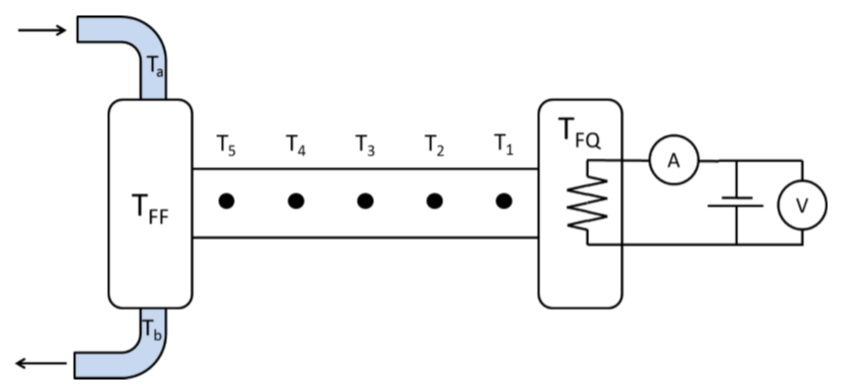
\includegraphics[width=180pt]{figura1.jpg}
\par\noindent {\scriptsize {\bf Figura 1:} Esquema da montagem para o regime estacionário}
\end{center}

\par A fonte quente é constituída por um circuito resistivo ligado a uma placa de cobre em contacto com a barra, sendo alimentado por uma fonte de tensão. A tensão e a corrente que percorrem a resistência podem ser determinadas através de um voltímetro e um amperímetro, sendo a potência fornecida à placa dada pela Lei de Joule:
\begin{equation} \label{PQ}
P_Q = U I
\end{equation}
\par A fonte fria é constituída por um sistema de refrigeração com água cuja temperatura à entrada e a saída é $T_a$ e $T_b$, respetivamente. Sendo assim, a potência cedida à fonte pode ser determinada pela equação \ref{PF}, em que $\phi$ é o caudal calculado pela expressão \ref{caudal}.
\begin{equation}\label{PF}
P_F = c \phi (T_b - T_a)
\end{equation}
\begin{equation} \label{caudal}
\phi = \frac{V_\rho}{\Delta t}
\end{equation}

\par Para analisar as transferências de calor entre a fonte quente e a barra, ao longo da barra, e entre a barra e a fonte fria, podemos considerar que o fluxo de calor é dado por:

\begin{equation} \label{RT}
\frac{dQ}{dt}=\frac{1}{R_T}\Delta T
\end{equation}

\par\nointent onde $\Delta T$ é a diferença de temperaturas entre a fonte quente e do início da barra, entre o início e o fim da barra ou entre o fim da barra e a fonte fria, consoante a resistência térmica $R_T$ que se pretenda determinar.

\par Podemos então considerar que entre a fonte quente e a barra se dissipa uma potência $P_{dQ}$ e que entre a barra e a fonte fria se dissipa uma potência $P_{dF}$. Temos então que o fluxo de calor na barra é dado pelas duas expressões:

\begin{equation} \label{A}
\frac{dQ}{dt}=P_Q-P_{dQ}
\end{equation}
\begin{equation} \label{B}
\frac{dQ}{dt}=P_F+P_{dF}
\end{equation}

\par\noindent onde, considerando que estas perdas se dão por condução, as potências dissipadas são

\begin{equation}
P_{dQ}=\alpha\PC{T_Q-T_{ar}}
\end{equation}
\begin{equation}
P_{dF}=\alpha\PC{T_F-T_{ar}}
\end{equation}

\par Somando as equações \eqref{A} e \eqref{B}, obtém-se:

\begin{equation} \label{T1}
\frac{dQ}{dt}=\frac{1}{2}\PC{P_Q+P_F+\alpha\PC{T_F-T_Q}}
\end{equation}

\par Utilizando dados referentes a duas tensões de alimentação diferentes, podemos obter $\alpha$ resolvendo a equação \eqref{alpha}, onde se utilizou a relação \eqref{k}.

\begin{equation} \label{alpha}
\frac{\frac{dQ_1}{dt}}{\frac{dQ_2}{dt}}=\frac{|\frac{dT}{dx}|_1}{|\frac{dT}{dx}|_2}=\frac{\PC{P_{Q1}+P_{F1}+\alpha\PC{T_{F1}-T_{Q1}}}}{\PC{P_{Q2}+P_{F2}+\alpha\PC{T_{F2}-T_{Q2}}}}
\end{equation}

\par Por último, é possível utilizar o valor de $\alpha$ na equação \eqref{T1} para estimar o fluxo de calor ao longo da barra para cada uma das tensões de alimentação.

\subsection*{Regime Variável}
Para a segunda parte considera-se o esquema da montagem experimental da figura 2, em que foi retirado o sistema de aquecimento, estando a barra apenas em contacto com o sistema de arrefecimento.

\begin{center}
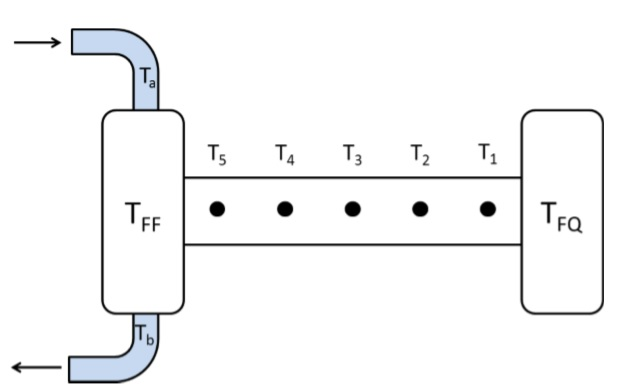
\includegraphics[width=180pt]{figura2.jpg}
\par\noindent {\scriptsize {\bf Figura 2:} Esquema da montagem para o regime variável}
\end{center}


\section{Dados Experimentais}

\subsection*{Estudo do regime estacionário}

\par Preparou-se a montagem da figura 1. Verificou-se que o caudal estava com o menor valor possível por forma a permanecer regular, escolheu-se uma tensão eficaz próxima dos $15V$, e esperou-se até que a maior diferença entre o máximo e o mínimo de temperaturas lida no programa fosse inferior a $0.5^\circ C$. Entretanto, mediu-se regularmente o caudal com o auxílio de uma proveta e de um cronómetro e aplicando a equação \eqref{caudal}. Atingido o regime estacionário, registaram-se os valores das várias temperaturas, assim como da tensão e da corrente de alimentação da unidade de aquecimento. 

\par Repetiu-se este processo para tensões próximas dos $20V$, e no final do estudo do regime variável para $5V$ e $10V$. Obtiveram-se os seguintes resultados:

{\small
\begin{center}
\begin{tabular}{ x{0.3cm} x{1.8cm} x{1.8cm} x{1.8cm} x{1.8cm} }
 & \multicolumn{4}{x{8.4cm}}{$\phi$ $(L/s)$} \tabularnewline
 & $V=5.02V$ & $V=10.06V$ & $V=15.07V$ & $V=19.99V$ \tabularnewline
\hline \hline
\multirow{3}{*}{$\phi_i$} & 0.888$\pm$0.006 & 0.894$\pm$0.006 & 0.901$\pm$0.006 & 0.930$\pm$0.006 \tabularnewline
 & 0.896$\pm$0.006 & 0.845$\pm$0.005 & 0.906$\pm$0.006 & 0.926$\pm$0.006 \tabularnewline
 & 0.900$\pm$0.006 & 0.859$\pm$0.006 & 0.907$\pm$0.006 & 0.940$\pm$0.006 \tabularnewline
$\overline{\phi}$ & 0.895$\pm$0.007 & 0.87$\pm$0.03 & 0.904$\pm$0.006 & 0.932$\pm$0.008 \tabularnewline
\end{tabular}
\par\noindent {\scriptsize {\bf Tabela 1:} Medições do caudal ao longo da realização da experiência}
\end{center}
}

{\small
\begin{center}
\begin{tabular}{ x{1.2cm} x{1.6cm} x{1.6cm} x{1.6cm} x{1.6cm} } 
$V$ $(V)$ & $5.02$ & $10.06$ & $15.07$ & $19.99$ \tabularnewline
\hline \hline
$T_Q$ $(^\circ C)$ & 35.1$\pm$0.4   & 58.2$\pm$0.6   & 68.4$\pm$0.7   & 92.3$\pm$0.9 \tabularnewline
$T_1$ $(^\circ C)$ & 25.4$\pm$0.2   & 33.0$\pm$0.2   & 50.48$\pm$0.09 & 74.90$\pm$0.08 \tabularnewline
$T_2$ $(^\circ C)$ & 24.80$\pm$0.05 & 31.29$\pm$0.05 & 46.73$\pm$0.06 & 68.0$\pm$0.1 \tabularnewline
$T_3$ $(^\circ C)$ & 24.15$\pm$0.05 & 29.21$\pm$0.05 & 42.46$\pm$0.06 & 59.7$\pm$0.1 \tabularnewline
$T_4$ $(^\circ C)$ & 23.35$\pm$0.04 & 27.27$\pm$0.05 & 38.09$\pm$0.04 & 50.57$\pm$0.06 \tabularnewline
$T_5$ $(^\circ C)$ & 22.88$\pm$0.05 & 25.78$\pm$0.05 & 34.3$\pm$0.1   & 44.3$\pm$0.2 \tabularnewline
$T_F$ $(^\circ C)$ & 21.68$\pm$0.05 & 22.77$\pm$0.05 & 26.42$\pm$0.08 & 31.8$\pm$0.2 \tabularnewline
$T_a$ $(^\circ C)$ & 21.61$\pm$0.07 & 21.23$\pm$0.07 & 21.28$\pm$0.08 & 21.74$\pm$0.09 \tabularnewline
$T_b$ $(^\circ C)$ & 22.0$\pm$0.2   & 22.63$\pm$0.4  & 24.5$\pm$0.5  & 27.7$\pm$0.7 \tabularnewline
$I$ $(A)$          & 0.44$\pm$0.01  & 0.87$\pm$0.01  & 1.30$\pm$0.01  & 1.73$\pm$0.01 \tabularnewline
\end{tabular}
\par\noindent {\scriptsize {\bf Tabela 2:} Grandezas registadas em regime estacionário}
\end{center}
}

\subsection*{Estudo do regime variável}

\par Estando o sistema no estado estacionário, com uma tensão de $20V$, desligou-se a fonte de tensão enquanto simultaneamente se isolou a barra da fonte quente com uma placa de esferovite e se iniciou o registo das temperaturas. Na figura 3 representam-se os dados obtidos, sendo que cada conjunto de pontos apresentado corresponde ao registado por um dos sensores de temperatura.

\begin{center}
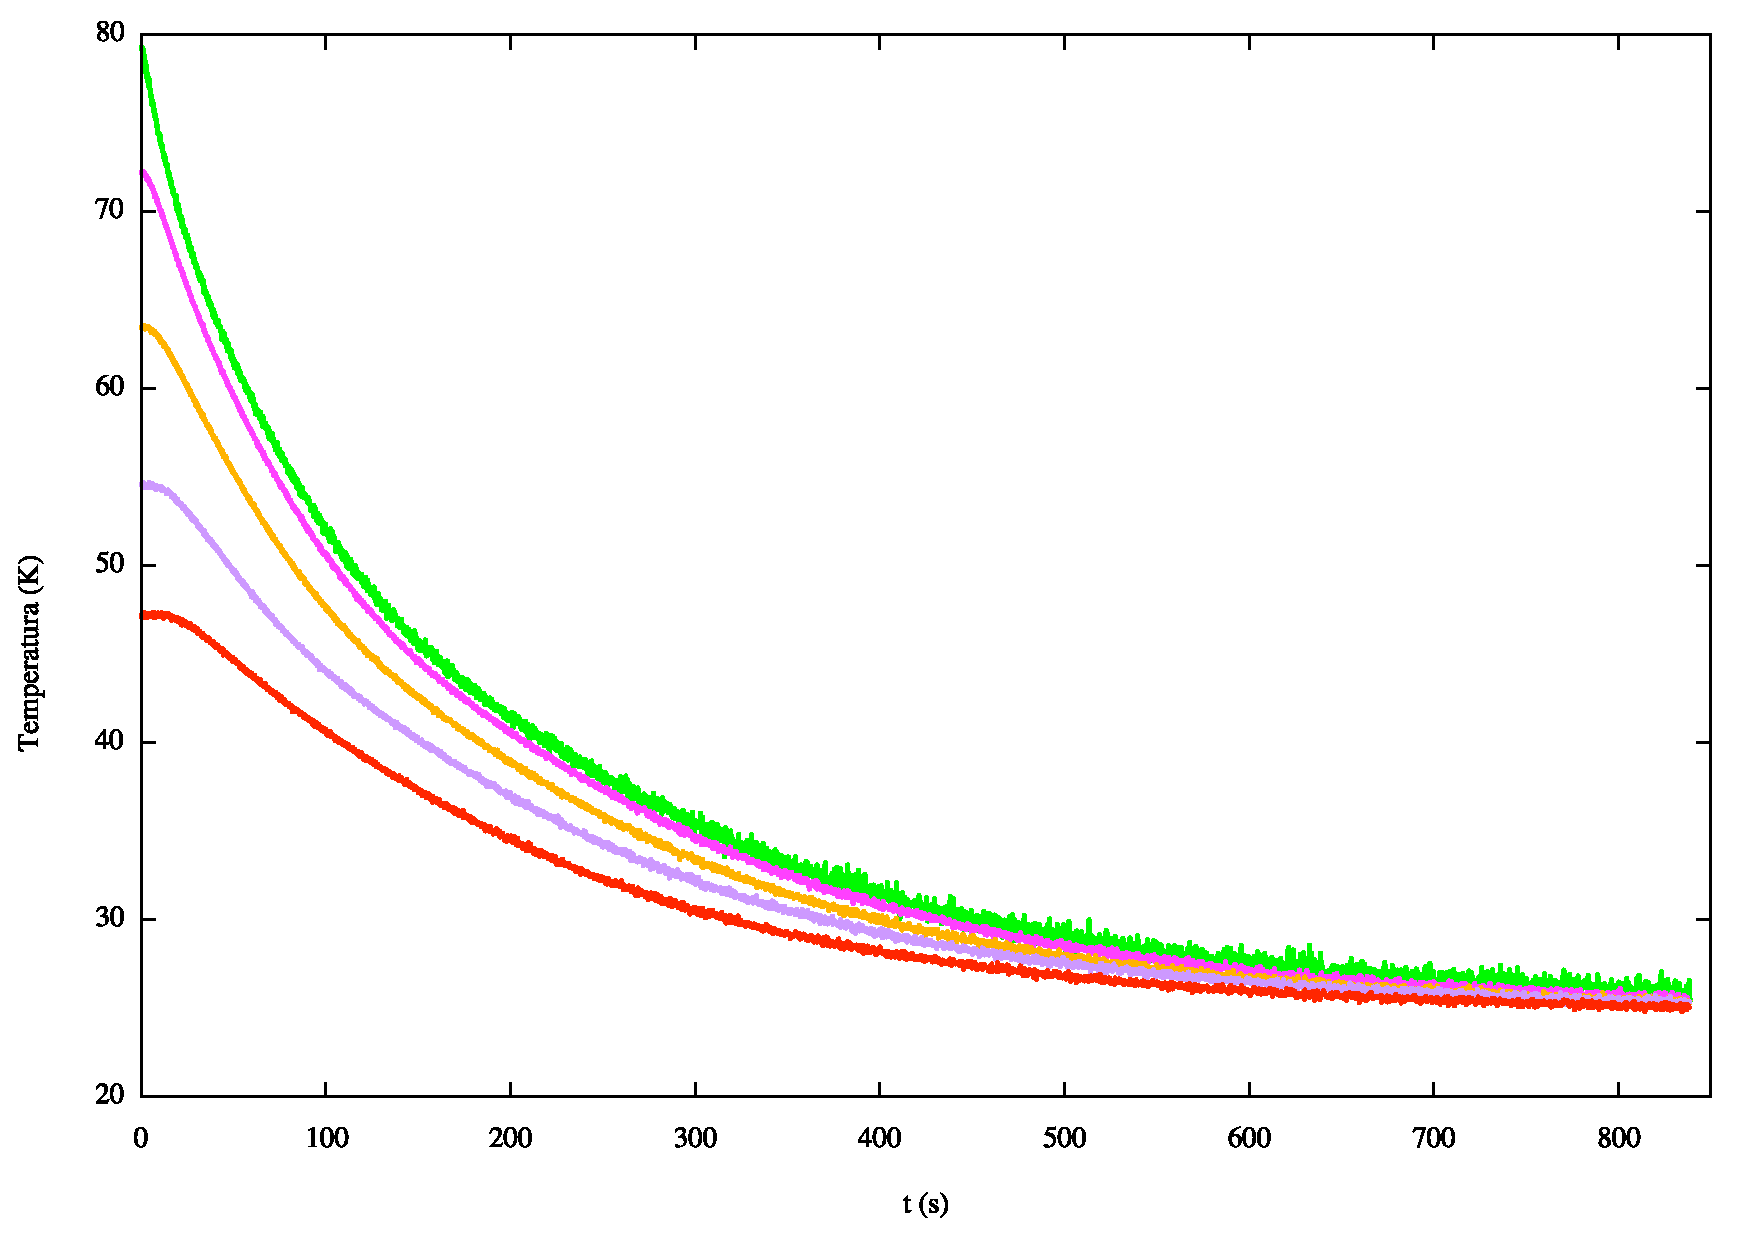
\includegraphics[width=200pt]{tras_2D.pdf}
\par\noindent {\scriptsize {\bf Figura 3}: Evolução da temperatura de diferentes posições da barra, no regime variável. As ordenadas na origem\footnote{pontos correspondentes a $t=0.015625s$} são, de cima para baixo, $79.4^\circ C$, $72.3^\circ C$, $63.5^\circ C$, $54.5^\circ C$ e $47.3^\circ C$. A curva verde corresponde ao sensor mais próximo da fonte quente}
\end{center}

\section{Análise e Discussão dos Resultados}

\subsection*{Estudo do regime estacionário}

\par Analisemos os dados das tabelas 1 e 2. No seguinte gráfico representa-se a variação da temperatura ao longo da barra de alumínio para as diferentes tensões e os respetivos ajustes da equação \eqref{ajuste1}.

\begin{center}
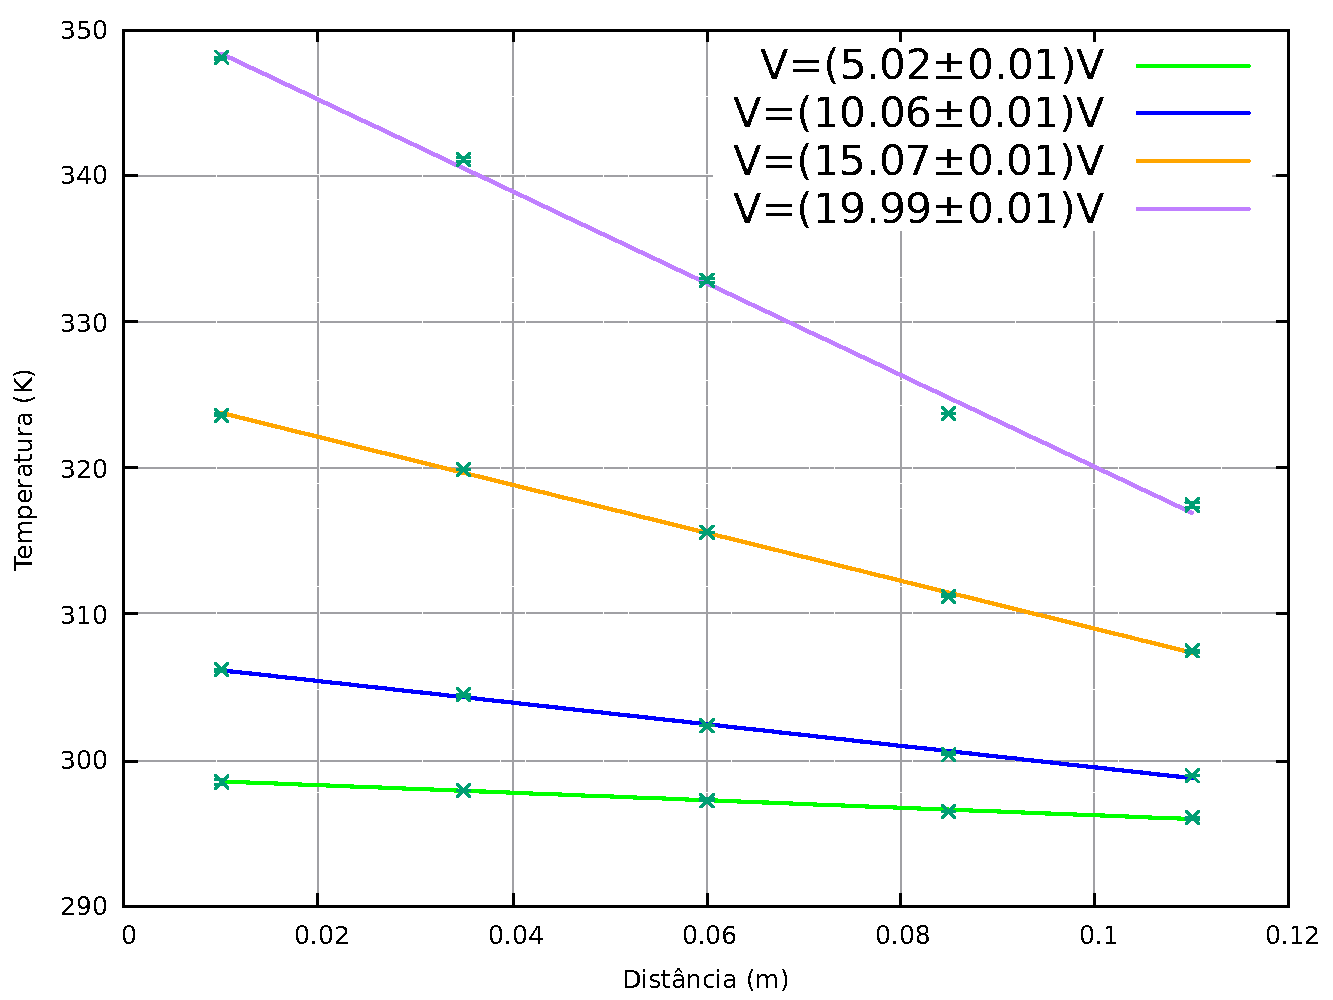
\includegraphics[width=220pt]{estacionario.pdf}
\par\noindent {\scriptsize {\bf Figura 4}: Variação da temperatura ao longo da barra. A verde representa-se o ajuste da equação \eqref{ajuste1} obtido pelo método dos mínimos quadrados para a tensão de $5.02V$, a azul para a tensão de $10.06V$, a cor de laranja para a tensão de $15.07V$ e a roxo para a tensão de $19.99V$}
\end{center}

\par Obtiveram-se os seguintes parâmetros de ajuste:

{\small
\begin{center}
\begin{tabular}{ x{1.5cm} x{1.3cm} x{1.3cm} x{1.3cm} x{1.3cm} } 
$V$ $(V)$ & $5.02$ & $10.06$ & $15.07$ & $19.99$ \tabularnewline
\hline \hline
$c_1$ $(Km^{-1})$ & -26$\pm$1     & -74$\pm$3     &  -164$\pm$3    & -314$\pm$11   \tabularnewline
$c_2$ $(K)$       & 298.8$\pm$0.1 & 306.9$\pm$0.2 & 325.4$\pm$0.2 & 351.5$\pm$0.8 \tabularnewline
\end{tabular}
\par\noindent {\scriptsize {\bf Tabela 3:} Parâmetros resultantes do ajuste da equação \eqref{ajuste1} representado na figura 3}
\end{center}
}

\par Por aplicação da equação \eqref{ajuste1}, é possível estimar a temperatura nas extremidades da barra: a temperatura da extremidade junto à fonte quente é $T_i=c_2$ e a temperatura da extremidade junto à fonte fria é $T_f=c_1l+c_2$, onde $l$ é o comprimento da barra. O gradiente de temperatura médio da barra é dado por $\frac{dT}{dx}=c_1$.

\par Utilizando as equações \eqref{PF} e \eqref{PQ}, foi possível determinar a potência fornecida pela fonte quente e a retirada pela fonte fria, bem como a diferença entre ambas que corresponde à potência dissipada:

{\small
\begin{center}
\begin{tabular}{ x{1.2cm} x{1.3cm} x{1.3cm} x{1.3cm} x{1.3cm} } 
$V$ $(V)$ & $5.02$ & $10.06$ & $15.07$ & $19.99$ \tabularnewline
\hline \hline
$P_Q$ $(W)$ & 2.21$\pm$0.06 & 8.8$\pm$0.2 & 19.6$\pm$0.2 & 34.6$\pm$0.3 \tabularnewline
$P_F$ $(W)$ & 1.6$\pm$0.8   & 5$\pm$2     & 12$\pm$2 & 23$\pm$4 \tabularnewline
$P_d$ $(W)$ & 0.6$\pm$0.9   & 4$\pm$2     & 7$\pm$2  &
12$\pm$4 \tabularnewline
\end{tabular}
\par\noindent {\scriptsize{\bf Tabela 4:} Potência fornecida pela fonte quente, potencia retirada pela fonte fria, e potência dissipada, para diferentes tensões}
\end{center}
}

\par Relativamente ao fluxo de calor e à determinação do valor da condutividade térmica do alumínio, deparamo-nos de imediato com um problema. Sabendo o valor da energia libertada pela fonte quente e daquela que chega à fonte fria, sabemos que a potência que atravessa a barra corresponderá à diferença entre estas descontando desse valor aquele que disser respeito à energia dissipada durante a propagação. Existem duas principais formas de lidar com este problema. A primeira consiste em admitir em primeira aproximação que a potência correspondente à barra é o valor médio entre a potência da fonte fria e da fonte quente, ou seja, que a potência que se dissiparia entre a fonte quente e a barra, por um lado, e entre a fonte fria e a barra, por outro, seria idêntica. Num sistema ideal tal poderia verificar-se. Todavia, neste caso, induzimos uma grande margem de erro pois tal não será necessariamente verdade (a dissipação irá de facto ocorrer predominantemente entre a fonte quente e a barra). Analisando este caso, verificamos os resultados seguidamente enunciados:

{\small
\begin{center}
\begin{tabular}{ x{1.9cm} x{1cm} x{1cm} x{1cm} x{1cm} } 
$V$ $(V)$ & $5.02$ & $10.06$ & $15.07$ & $19.99$ \tabularnewline
\hline \hline
$P_B\equiv\frac{dQ}{dt}$ $(W)$ & 1.9$\pm$0.5 & 6.9$\pm$0.9 & 16$\pm$2   & 29$\pm$2 \tabularnewline
$k$ $(Wm^{-2}K)$ & 186$\pm$48  & 234$\pm$38  & 241$\pm$21 & 228$\pm$22 \tabularnewline
$\delta_\text{exatidão} (\%)$ & 21.6 &1.4 & 1.7 & 3.7\tabularnewline
$\delta_\text{precisão} (\%)$ & 25.2 & 16.2 & 8.4 & 9.6\tabularnewline
\end{tabular}
\par\noindent {\scriptsize{\bf Tabela 5:} Resultados tomando como potência da barra a média das potências fria e quente.}
\end{center}
}

\par Notamos de imediato que uma maior tensão permite uma muito melhor aproximação do valor desejado para a condutividade térmica - de facto, para 15.07V e 19.99V o desvio à precisão é extremamente inferior ao para 5.02V. Todavia, o desvio à precisão permanece de tal modo elevado que mesmo nos casos em que o valor obtido é extremamente concordante com o real (10.06, 15.07V e 19.99V) o erro da experiência dificulta as conclusões obtidas - embora todos os valores se encontrem dentro do desvio de precisão permitido. É forçoso ainda notar a má qualidade do caso 5.02V. Tal resulta do sistema ainda não ter atingido o equilíbrio térmico, fruto da experiência ter sido realizada passando da tensão mais elevada para esta directamente. Assim, embora a maioria do sistema tenha tido possibilidade de atingir equilíbrio térmico, o mesmo não ocorreu para a fonte quente, dissipando-se muito mais energia do que esperado e consequentemente induzindo um valor de k significativamente mais baixo do que o real. Isto será suportado posteriormente quando for efectuada a análise das resistências térmicas.

\par Uma outra forma de lidar com este problema seria considerar que a barra se encontra perfeitamente isolada e que a dissipação se dará por transferência de energia para o ar exterior da forma delineada previamente na introdução. Quanto a este, verificámos para os valores de tensão cujo estudo consistia o âmbito inicial do trabalho que os resultados correspondem a:

{\small
\begin{center}
\begin{tabular}{ x{1.9cm} x{1.2cm} x{1.2cm} x{1.2cm} x{1cm} } 
$V$ $(V)$ & $5.02$ & $10.06$ & $15.07$ & $19.99$ \tabularnewline
\hline \hline
$P_B\equiv\frac{dQ}{dt}$ $(W)$ & 2$\pm$3 & 7$\pm$6 & 17$\pm$7   & 29$\pm$11 \tabularnewline
$k$ $(Wm^{-2}K)$ & 202$\pm$240 & 249$\pm$216 & 249$\pm$114 & 234$\pm$93 \tabularnewline
$\delta_\text{exatidão} (\%)$ & 14.8  & 5.1 & 5.1 & 1.2 \tabularnewline
$\delta_\text{precisão} (\%)$ & 118 & 86 & 46 & 39 \tabularnewline
\end{tabular}
\par\noindent {\scriptsize{\bf Tabela 6:} Resultados tomando como potência da barra a hipótese apresentada}
\end{center}
}

\par Assim, podemos constatar que este método constitui uma aproximação pior do que a anterior. De facto, embora os valores obtidos sejam concordantes com os anteriores, os erros são de tal forma elevados que invalidam conclusões passíveis de se extrairem. Notamos que este erro surge maioritariamente do erro de $T_b$, o qual se propaga posteriormente através da potência da fonte fria. Contudo, verificamos também que um aumento de voltagem neste caso provoca uma demarcada melhoria quer no erro inerente à experiência quer no desvio ao valor real. Devemos ainda chamar a atenção para a volatilidade dos valores de k obtidos para esta última abordagem - de facto, uma alteração de uma centésima no valor do quociente entre os gradientes de temperatura para a barra provoca uma variação na ordem das unidades na condutividade térmica - ora, considerando que os gradientes possuem valores na ordem das centenas, notamos que a menor perturbação nos resultados obtidos modifica de forma drástica o valor de k. Por conseguinte, temos que considerar este método demasiado sensível a erros inerentes à experiência para ser útil o seu emprego (embora em muito boas condições de execução - nomeadamente, diferenças de potencial muito mais elevadas, correspondesse a um método ideal). Notamos ainda que, para minimizar os erros, a constante de dissipação $\alpha$ foi calculada para todos os possíveis pares de valores de voltagem - ignorando-se aqueles que correspondem ao caso 5.02V visto este não se encontrar em equilíbrio térmico. 

\par Relativamente ao cálculo das resistências térmicas, optou-se pela utilização dos valores resultantes da potência média visto os cálculos efectuados a partir destes apresentarem um menor desvio em relação ao valor real da condutividade térmica do alumínio. Para estes verificaram-se os seguintes valores:

{\small
\begin{center}
\begin{tabular}{ x{1.8cm} x{1.3cm} x{1.3cm} x{1.3cm} x{1.3cm} } 
$V$ $(V)$ & $5.02$ & $10.06$ & $15.07$ & $19.99$ \tabularnewline
\hline \hline
$R_Q$ $(KW^{-1})$ & 4.2$\pm$0.3 & 2.79$\pm$0.03 & 0.82$\pm$0.04 & 0.40$\pm$0.05 \tabularnewline
$R_B$ $(KW^{-1})$ & 1.3$\pm$0.4 & 1.0$\pm$0.2 & 1.01$\pm$0.08 & 1.07$\pm$0.07 \tabularnewline
$R_F$ $(KW^{-1})$ & 0.5$\pm$0.4 & 0.4$\pm$0.2 & 0.5$\pm$0.1 & 0.4$\pm$0.1 \tabularnewline
\end{tabular}
\par\noindent {\scriptsize{\bf Tabela 7:} Resistências térmicas da barra e da junção da barra com os sistemas de aquecimento e arrefecimento, para diferentes tensões}
\end{center}
}

\par É fácil observar que enquanto que $R_F$ e $R_B$ se comportam como esperado, mantendo-se constante dentro da margem de incerteza permitida, o mesmo não acontece para a resistência quente. De facto, embora o valor para 5V seja ignorável visto não se encontrar em equilíbrio térmico, como previamente enunciado, a verdade é que mesmo para os restantes valores de tensão existe uma enorme discrepância - não contida dentro da margem de erro - no tocante à resistência térmica. Na realidade, torna-se impossível concluir sobre o seu possível valor, visto todos serem distintos. Tal resultará provavelmente do facto de a fonte quente necessitar de mais tempo até atingir o equilíbrio térmico - embora o erro da temperatura desta fonte se encontre dentro do valor permitido para considerar equilíbrio, provavelmente necessitaria de mais tempo para permitir que esta temperatura descesse. 

\subsection*{Estudo do regime transitório}

\par Relativamente ao estudo do regime transitório, começou-se por efectuar um fit dos dados experimentais de acordo com a equação (9), deixando enquanto parâmetros livres $\chi$ e $T_Q$. Assim, obteve-se o seguinte gráfico:

\begin{center}
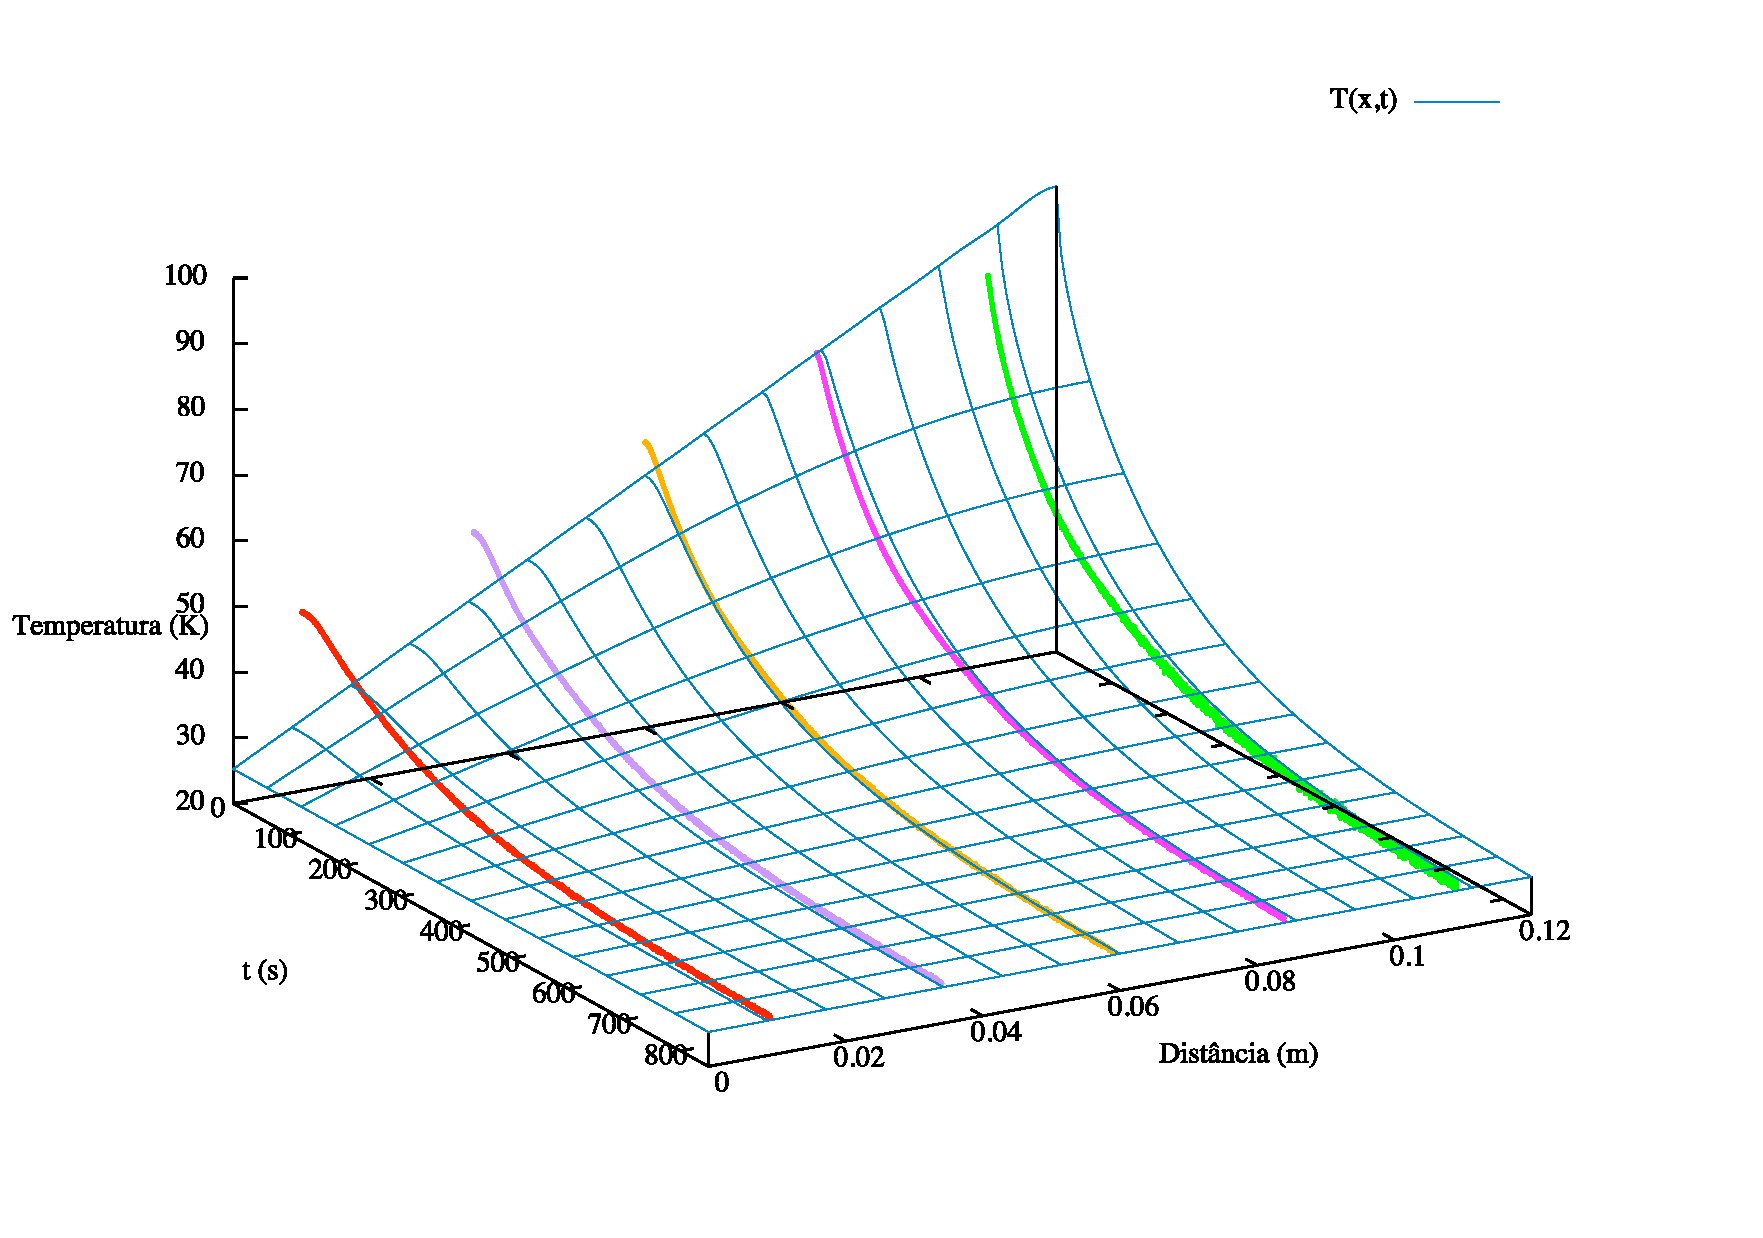
\includegraphics[width=220pt]{trans_nao_ajustado.pdf}
\par\noindent {\scriptsize {\bf Figura 5}: Variação da temperatura nos 5 pontos estudados da barra ao longo do tempo}
\end{center}

{\small
\begin{center}
\begin{tabular}{ x{2.5cm} x{2.5cm} } 
\hline \hline
$\chi(m^{2}s^{-1})$ & $(2.21\pm0.01)\times10^{-3}$ \tabularnewline
$T_2(K)$  & $91.5\pm0.2$ \tabularnewline
\hline \hline
\end{tabular}
\par\noindent {\scriptsize {\bf Tabela 3:} Parâmetros resultantes do ajuste da equação (9) representado na figura 5}
\end{center}
}

\par Para este, efectuando os cálculos a partir dos parâmetros de ajuste, obtem-se um valor para a condutividade térmica de $k=77.4\pm0.1 Wm^{-2}K$, que apresenta uma desvio à exactidão de $67\%$ e um desvio à precisão de apenas $0.13\%$. De facto, este resultado é de muito má qualidade: todavia, devemos ter em conta que as condições fronteira impostas não são as correctas. De facto, a barra não irá estar isolada nas suas extremidades. Para se obter um ajuste correcto, devemos considerar um fit no qual tenhamos em conta uma barra maior que será, para todos os efeitos, o acoplamento da barra e das fontes. Assim, considerou-se um factor de ajuste adicional correspondente a $(x-a)$. Para este, obteve-se os seguintes resultados:

\begin{center}
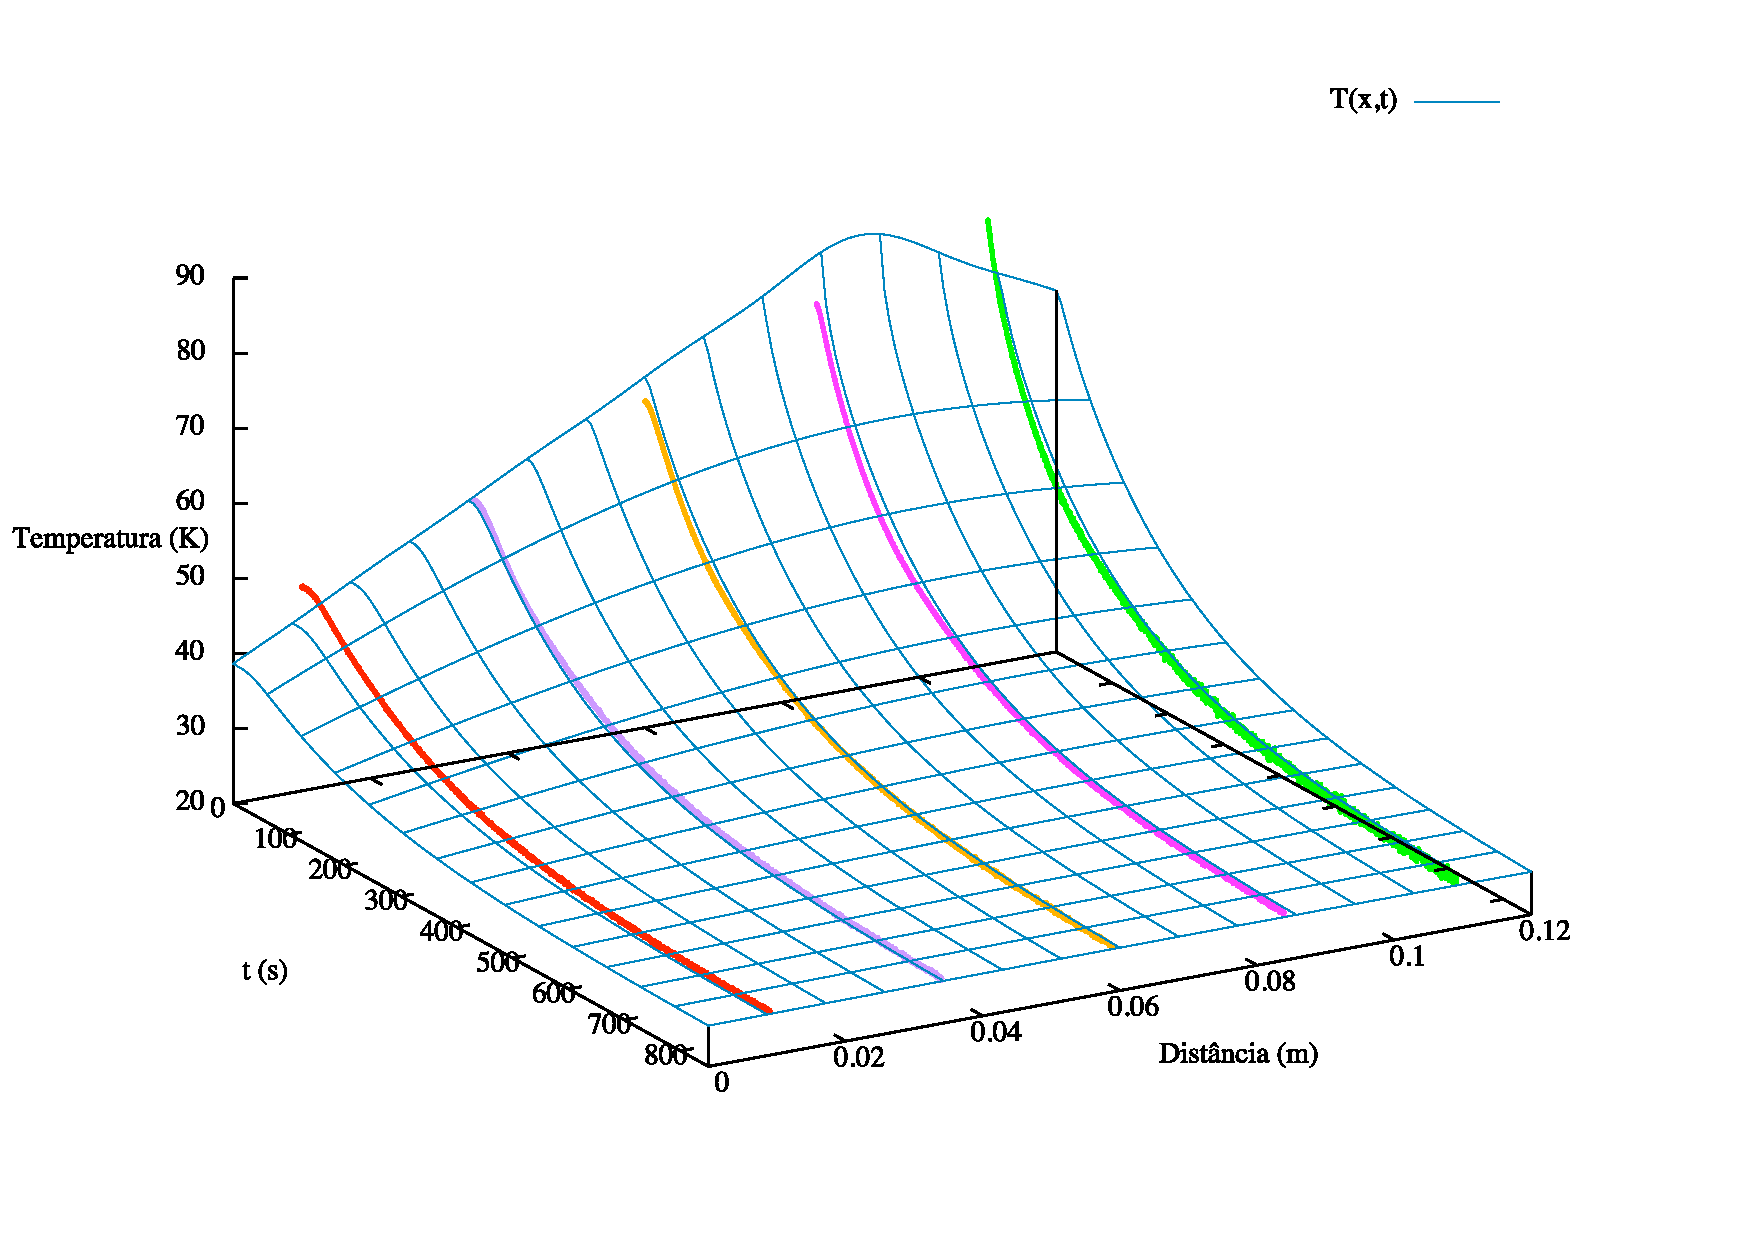
\includegraphics[width=220pt]{trans_ajustado.pdf}
\par\noindent {\scriptsize {\bf Figura 6}: Variação da temperatura nos 5 pontos estudados da barra após feita a correcção para a distância}
\end{center}

{\small
\begin{center}
\begin{tabular}{ x{3cm} x{3cm}} 
\hline \hline
$\chi(m^{2}s^{-1})$ & $(2.139\pm0.004)\times10^{-3}$ \tabularnewline
$T_2(K)$ & $81.35\pm0.05$ \tabularnewline $a(m)$ & $(2.8\pm0.008)\times10^{-2}$ \tabularnewline
\hline \hline
\end{tabular}
\par\noindent {\scriptsize {\bf Tabela 8:} Parâmetros resultantes do ajuste da equação (9) representado na figura 6}
\end{center}
}

\par Assim, podemos verificar que o valor obtido desta feita será $k=117\pm13 Wm^{-2}K$, que apresenta um desvio à exactidão de $51\%$ e um desvio à precisão de $11\%$. Notamos desde logo que, embora melhor, mesmo este ajuste não apresenta a qualidade desejada. Tal resultará do valor de a - apesar do fit ser bom, o valor de a é inferior ao que se esperaria: a distância entre as fontes e a barra é certamente maior que 1.4cm, que é o que a implicaria neste caso. Isso implica um valor de k inferior àquele que seria o real, o que de facto se verifica.

\par Por fim, calculou-se directamente a partir da forma diferencial da equação (5) através da determinação numérica das derivadas, efectuando-se o seu fit. Este encontra-se apresentado de seguida:

\begin{center}
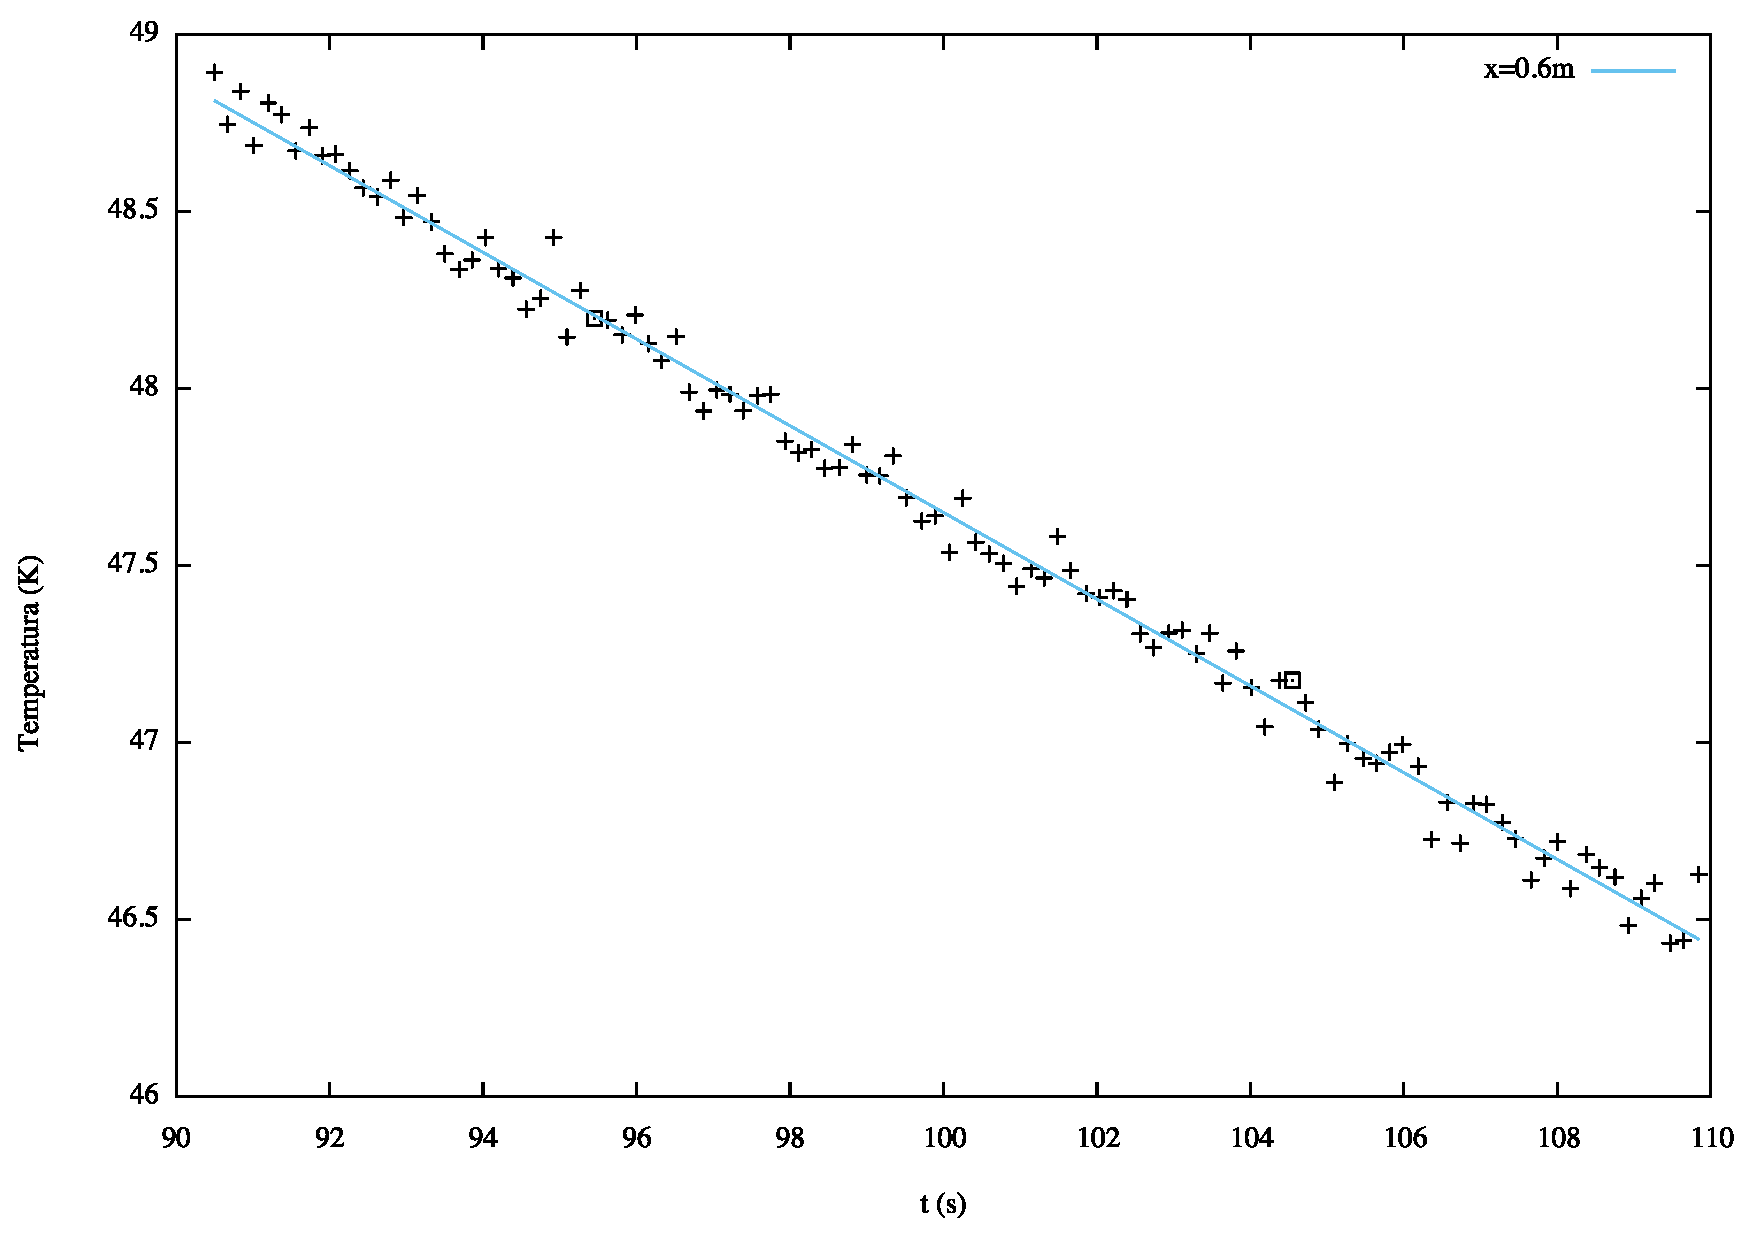
\includegraphics[width=180pt]{xfixo.pdf}
\par\noindent {\scriptsize {\bf Figura 7}: Variação da temperatura ao longo do tempo para um dado x fixo ao longo do tempo. Os pontos representados com um quadrado são $(95.5s,48.2K)$ e $(104.4s,47.2K)$}
\end{center}

\begin{center}
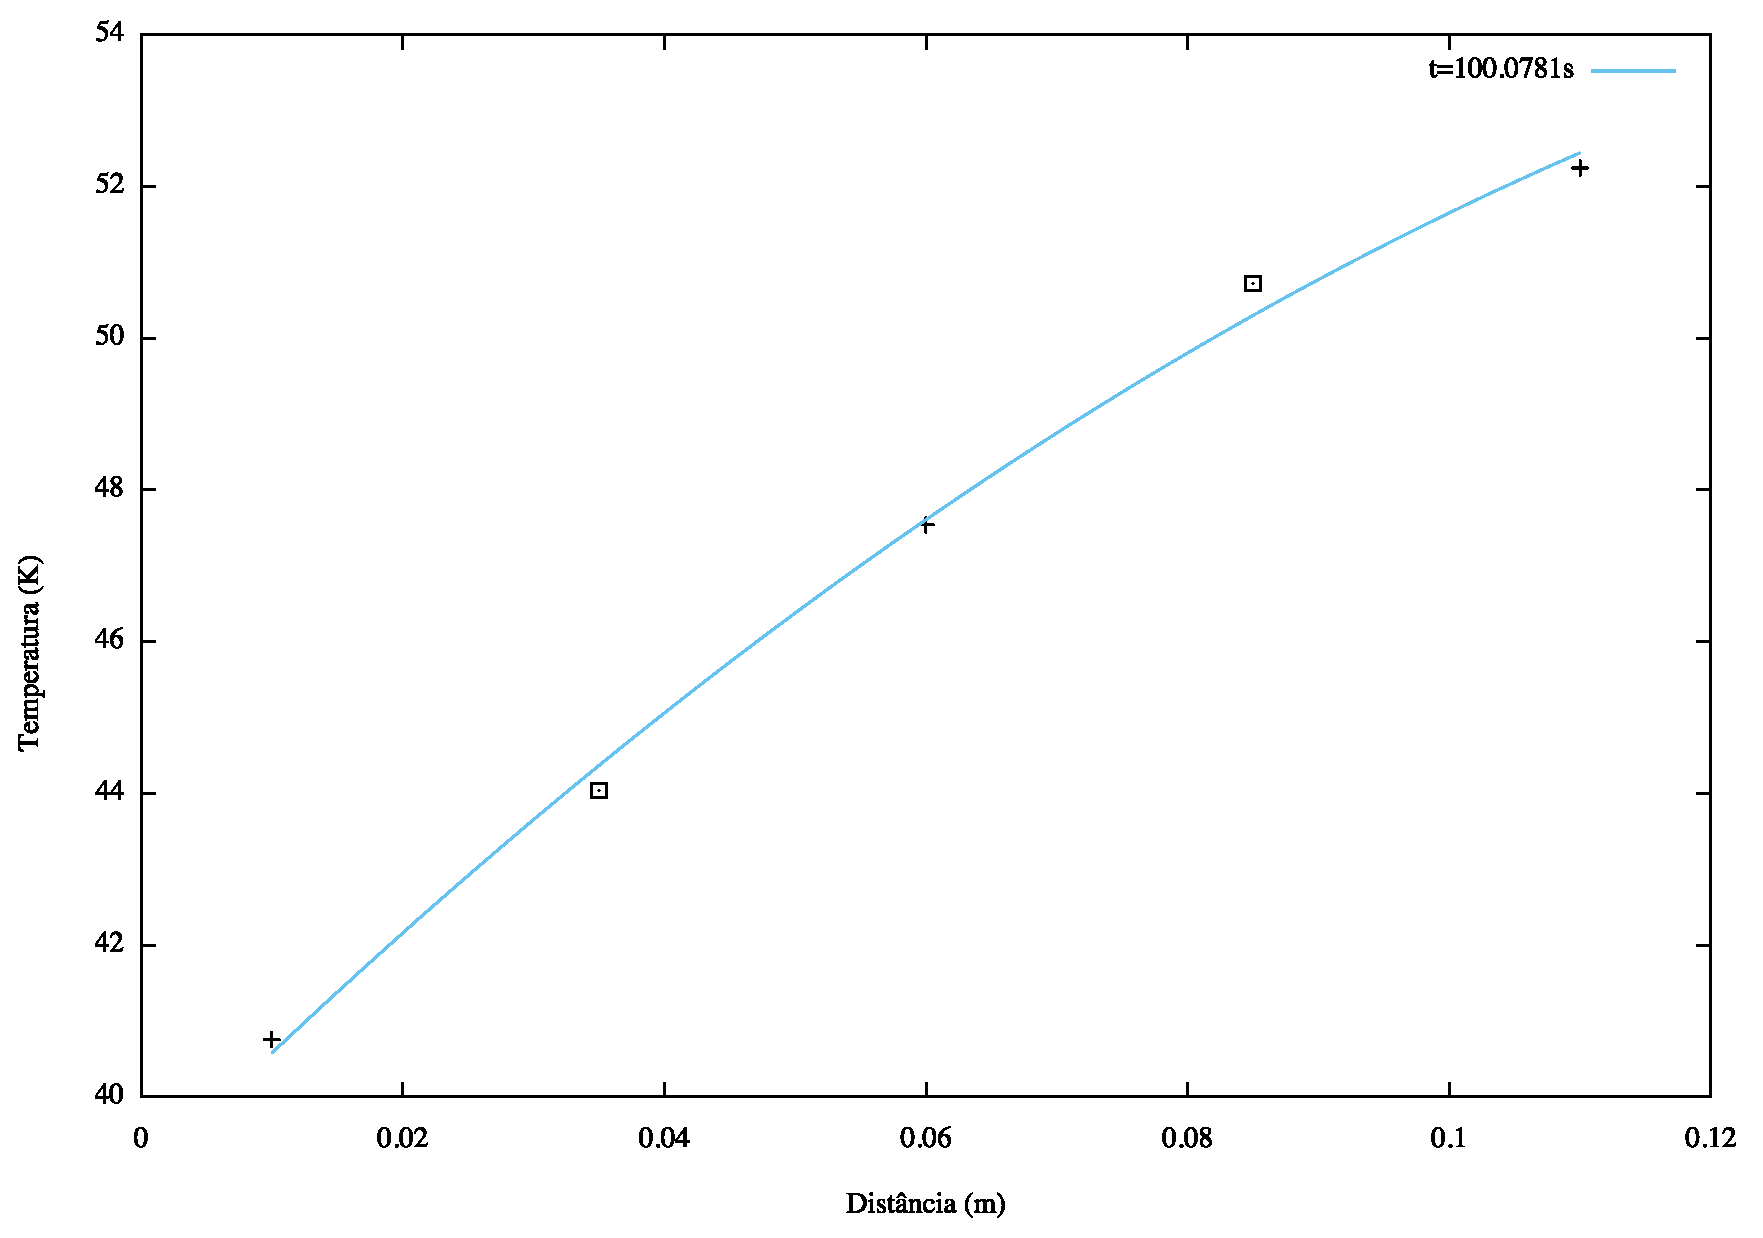
\includegraphics[width=180pt]{tfixo.pdf}
\par\noindent {\scriptsize {\bf Figura 8}: Variação da temperatura ao longo da barra para um dado valor de tempo. Os pontos representados com um quadrado são $(0.085m,50.7K)$ e $(0.035m,44.0K)$}
\end{center}

{\small
\begin{center}
\begin{tabular}{ x{3cm} x{3cm}} 
\hline \hline
$\frac{\partial T}{\partial t}$ $(Ks^{-1})$ & $0.1225\pm0.0002$ \tabularnewline 
$\frac{\partial^2 T}{\partial x^2}$ $(Km^{-2})$ & $878\pm132$ \tabularnewline
\hline \hline
\end{tabular}
\par\noindent {\scriptsize {\bf Tabela 9:} Valores calculados a partir dos ajustes das figuras 7 e 8}
\end{center}
}

\par Agora, por substituição directa, facilmente se verifica que o valor da condutividade térmica será $k=339\pm166 Wm^{-2}K$, o qual apresenta um desvio à exactidão de 37$\%$ e um desvio à precisão de $49\%$. Embora o resultado verificado seja melhor do que o previamente obtido, notamos que ainda assim existe um desvio à exactidão e à precisão extremamente elevados, indiciando a má qualidade do processo. De facto, a principal fonte de erro vem do elevado valor dos erros inerentes ao fit que, apesar de baixos por si, quando multiplicados pela constante $\rho c=2.43\times10^6$ torna-se bastante elevado

\section{Conclusão}
\par Após a realização desta experiência podemos verificar que o estudo do regime estacionário é muito mais fiável e simples do que o estudo do regime transiente, o qual induz valores extremamente díspares entre si e errados da condutividade térmica, fruto das condições de fronteira não serem idealmente determinadas e de o ajuste a efectuar ser como tal sujeito a erros e aproximações. Notámos todavia que os valores da condutividade térmica determinados através do estudo do regime transitório são extremamente satisfatórios, apesar de serem caracterizados por uma incerteza um pouco mais elevada do que seria ideal. 

\begin{thebibliography}{9}

\bibitem{guia} Guia de objetivos do trabalho, Professor João Figueirinhas
\bibitem{apontamentos} Apontamentos das aulas teóricas

%\bibitem{site} Wikipedia, the free encyclopedia - Thermoelectric effect. [Online] Available from: \url{http://en.wikipedia.org/wiki/thermoelectric\_effect}
\end{thebibliography}

\end{multicols}
 


\end{document}